\documentclass[10pt,a4paper]{article}
\usepackage[utf8]{inputenc}
\usepackage[russian]{babel}
\usepackage{amsmath}
\usepackage{amsfonts}
\usepackage{amssymb}
\usepackage{graphicx}
\usepackage{placeins}
\author{Анастасия Тарасова}
\title{Отчет по лабораторной работе №5\\ Проект OWASP WebGoat}
\begin{document}
\maketitle
\section{Цель работы}
Изучить описание деятельности самых распространенных веб-уязвимостей согласно рейтингу OWASP.
\section{Ход работы}

\paragraph{Исследование 10 самых распространенных web-уязвимостей по рейтингу OWASP} 

\begin{enumerate}
\item \textbf{Injection} Атака на интепритатор машины-цели, позволяя выполнять произвольный код от ее имени. Чаще всего встрачаются в SQL, LDAP, Xpath, или NoSQL запросах, парсерах xml, аргументах программ и т.д.

\item \textbf{Broken Authentication and Session Management} Атака на уязвимости систем авторизации и управления сессиями с целью кражи и/или выполнения каких либо действий от чужого имени.

\item \textbf{Cross-Site Scripting} Атака на браузер путем подмены загружаемых скриптов. В результате злоумышлиниками может быть получена почти любая информация.

\item \textbf{Insecure Direct Object References} Суть атаки - изменение некого объекта, используемого в авторизированной сессии. Пример: 
\begin{verbatim}
String query = "SELECT * FROM accts WHERE account = ?";
PreparedStatement pstmt = connection.prepareStatement(query , … );

pstmt.setString( 1, request.getParameter("acct")); <<<<<

ResultSet results = pstmt.executeQuery( );
\end{verbatim}

Изменение параметра позволит отправлять измененные запросы от имени авторизированного пользователя.

\item \textbf{Security Misconfiguration} Ошибки в конфигурации. Атакующий может получить доступ к файлам, акаунтам, системе и т.д.

\item \textbf{Sensitive Data Exposure} Кража ценной/личной информации. Атака сложна если используется шифрование. В таком случае данные крадутся косвенными методами: на стороне клиента, когда данные уже рашифрованы, man-in-the-middle атака и другими способами.

\item \textbf{Missing Function Level Access Control} Доступ неавторизированного пользователя к привелегированным функциям. 
Пример: 

\begin{verbatim}
http://example.com/app/getappInfo
http://example.com/app/admin_getappInfo <<<<
\end{verbatim}

Доступ к функции admin\_getappInfo должен иметь только администратор. Соответственно, если пользователь, не являющийся администритором получает доступ к данной функции - это уязвимость.

\item \textbf{Cross-Site Request Forgery} Атака путем выполнения запросов к некоторому защищенному ресурсу от его имени авторизованного пользователя. Недостаток - атакующий \textbf{НЕ} может перехватить ответ от ресурса. В этом случае вводят так называемые CSRF-токены: каждый последующий пакет от клиента содержит токен, полученный в пердыдущем ответе сервера.

\item \textbf{Using Components with Known Vulnerabilities} Атака на уязвимый компонет системы, выявленный в результате сканирования.

\item \textbf{Unvalidated Redirects and Forwards} Скрытые ссылки в картинках, фреймах и т.д., ведущих на доверенный сайт. Позволяет произвести любой запрос.
Пример:
\begin{verbatim}
http://www.example.com/redirect.jsp?url=evil.com
\end{verbatim}
\end{enumerate}

\paragraph{Подготовка}
Скачаем WebGoat, OWASP Mantra, OWASP Zed Attack Proxy. 

Запустим уязвимое приложение WebGoat (рисунок 1).
\FloatBarrier
\begin{figure}[h!]
\centering
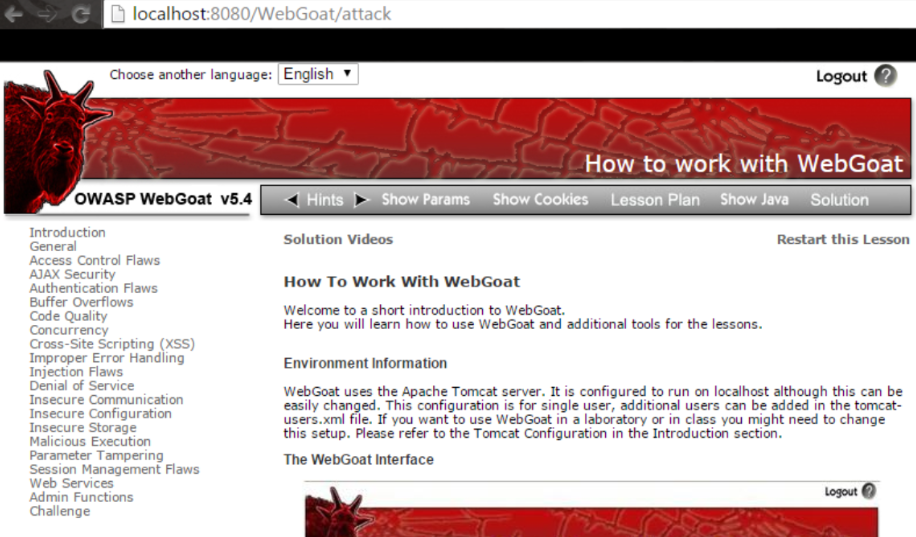
\includegraphics[scale=0.5]{1}
\caption{Запуск WebGoat в браузере Mantra}
\end{figure}
\FloatBarrier
Настроим инструмент Mantra для использования ZAP (сканера безопасновати) в качестве прокси-сервера (рисунок 2).
\FloatBarrier
\begin{figure}[h!]
\centering
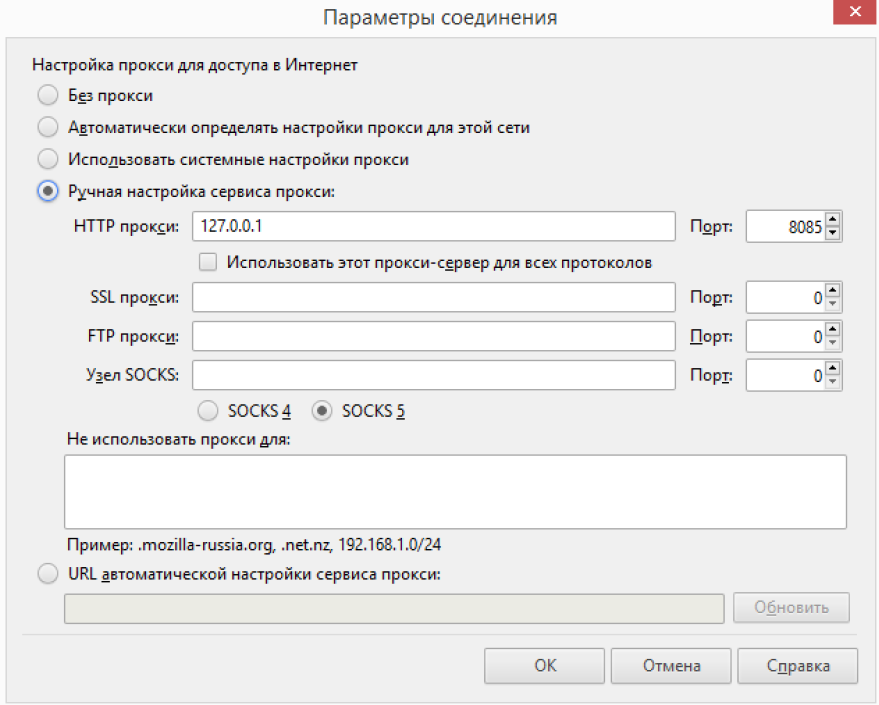
\includegraphics[scale=0.5]{2}
\caption{Настройка прокси-сервера}
\end{figure}
\FloatBarrier
Запустим ZAP и видим, что на панели сайтов появился WebGoat и перехват запросов(рисунок3).
\FloatBarrier
\begin{figure}[h!]
\centering
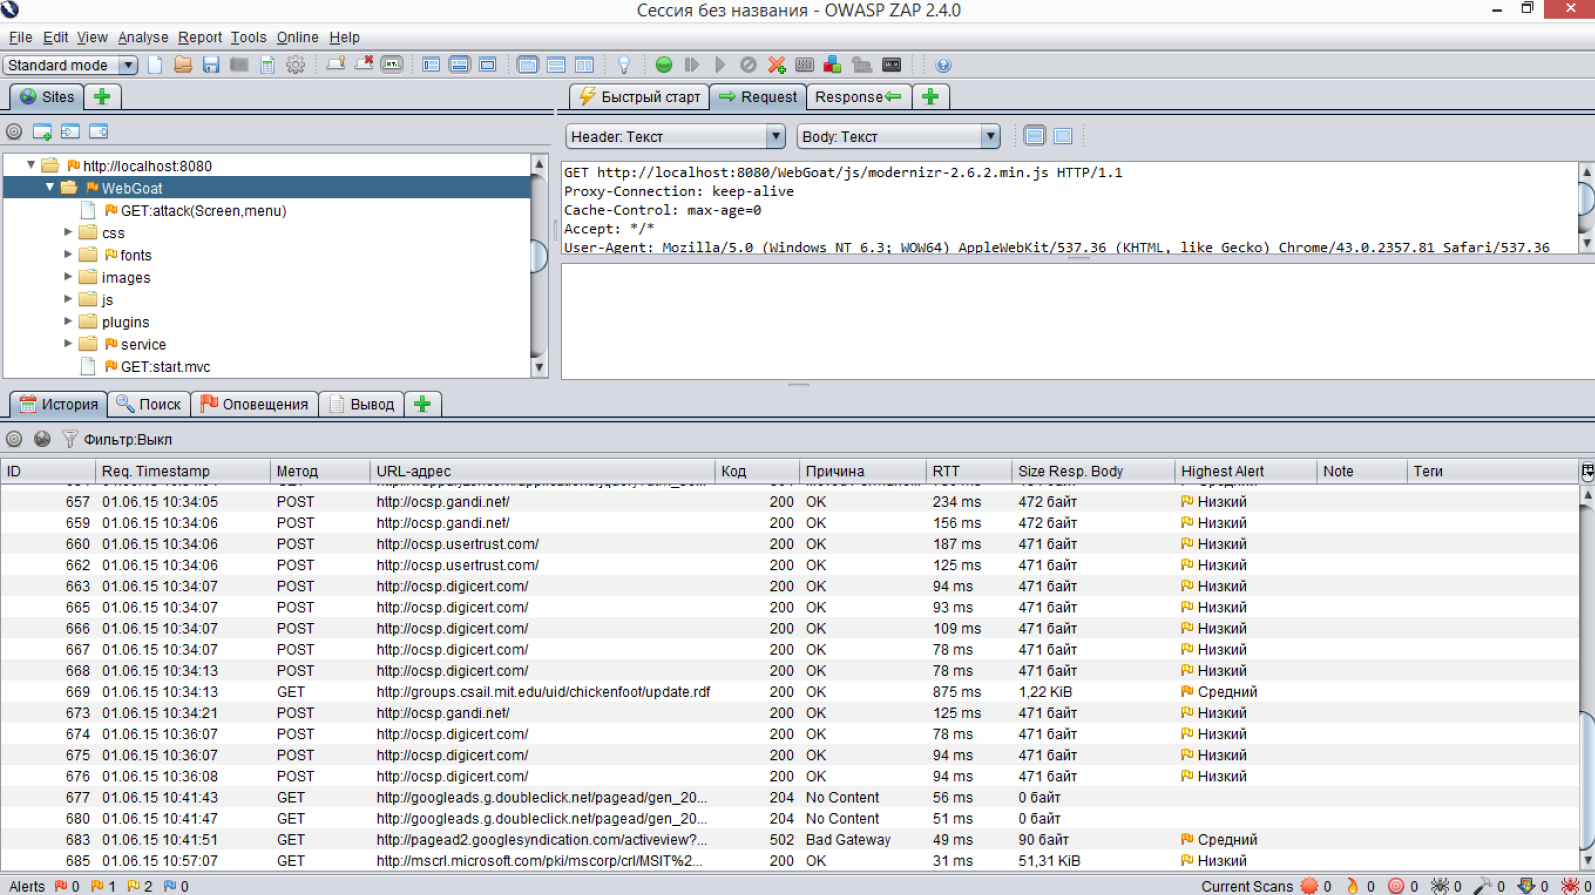
\includegraphics[scale=0.4]{3}
\caption{Работа ZAP}
\end{figure}
\FloatBarrier
Зададим Http Basics, введем своем имя в поле и поставим ZAP в режим прослушивания (рисунок 4).
\FloatBarrier
\begin{figure}[h!]
\centering
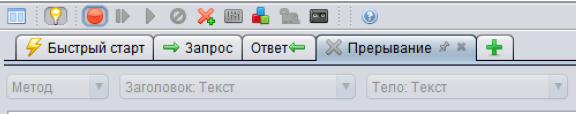
\includegraphics[scale=0.4]{4}
\caption{ZAP в режиме прослушивания}
\end{figure}
\FloatBarrier
Отправим данные (GO!) и увидим, что был перехвачем POST запрос (рисунок 5.)
\FloatBarrier
\begin{figure}[h!]
\centering
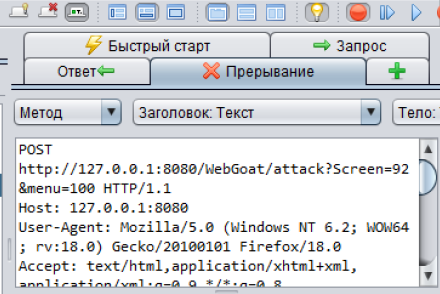
\includegraphics[scale=0.4]{5}
\caption{ZAP перехватил POST запрос}
\end{figure}
\FloatBarrier
\end{document}